
\chapter{Declaration of AI Compliance}
\label{app:AI_compliance}
This thesis follows the NMBU Guidelines for the Use of Generative Artificial Intelligence (AI). In accordance with the university’s standards for academic integrity and transparency, the following disclosure outlines the role of AI-based programs, specifically ChatGPT, Claude, Gemini, and Grok, in the development of this work

Generative AI platforms were employed as a research method to assist in designing analytical frameworks and identifying relevant academic literature. To ensure the reliability of the research and mitigate the risk of fictitious sources, we verified AI-suggested references manually against recognized scientific databases to confirm they are authentic. No AI-generated text served as a primary source for factual information; all findings are grounded in verified research as represented in the text and bibliography.  

Additionally, AI tools provided writing and coding support through language polishing and code refinement. This assistance was used to improve the clarity of the manuscript and the efficiency of the vehicle classification and tracking scripts. As required by NMBU regulations, we maintain full responsibility for the final text. All work was conducted with full transparency and adheres to the academic norms for honesty and accountability.

\chapter{GitHub links}
\label{app:github_links}
\begin{table}[H]
\centering
\caption{Repository link and commit hash.}
\label{tab:github_links}
\begin{tabular}{p{4.8cm} p{4.4cm} p{3.4cm}}
\toprule
\textbf{Title} & \textbf{Link} & \textbf{Commit} \\
\midrule
Master thesis repository & \href{https://github.com/sondreehaugen/Master_thesis}{GitHub link} & ecb447b \\
\bottomrule
\end{tabular}
\end{table}

\chapter{FFmpeg script}
\label{app:ffmpeg}
This shell command used to download video data in 5 minute segments for 1 hour.

\begin{minted}[fontsize=\small,breaklines,frame=single]{bash}
# Set output directory (edit as needed)
OUT_DIR="/path/to/footage/5min"

mkdir -p "$OUT_DIR"

ffmpeg -loglevel warning \
       -stats \
       -fflags +genpts \
       -t 3600 \
       -i "https://kamera.vegvesen.no/public/1229050_1/manifest.m3u8" \
       -c copy \
       -f segment \
       -segment_time 300 \
       -reset_timestamps 1 \
       -movflags +faststart \
       "$OUT_DIR/Fv587_Haukeland_1229050_$(date +%Y%m%d_%H%M%S)_%02d.mp4"
\end{minted}


\chapter{YOLO26 Hyperparameters}
\label{app:hyperparameters}

\begin{table}[H]
\caption{Default training hyperparameters (from args.yaml) used for YOLO26n and YOLO26m models.}
\centering
\small
\begin{tabular}{ll|ll}
\hline
Parameter & Value & Parameter & Value \\
\hline
epochs & 100 & hsv\_s & 0.7 \\
batch & 16 & hsv\_v & 0.4 \\
imgsz & 640 & translate & 0.1 \\
patience & 20 & scale & 0.5 \\
lr0 & 0.01 & fliplr & 0.5 \\
lrf & 0.01 & erasing & 0.4 \\
momentum & 0.937 & mosaic & 1.0 \\
weight\_decay & 0.0005 & mixup & 0.0 \\
warmup\_epochs & 3.0 & close\_mosaic & 10 \\
warmup\_momentum & 0.8 & iou & 0.7 \\
box & 7.5 & max\_det & 300 \\
cls & 0.5 & optimizer & auto \\
dfl & 1.5 & split & val \\
hsv\_h & 0.015 & seed & 42 \\
\hline
\end{tabular}
\label{tab:yolo_hyperparameters}
\end{table}


% --- Appendix B ---
\chapter{Validation Metrics}
\label{app:val_metrics}
This appendix contains the validation set results for the YOLO26 models.

\begin{table}[H]
\centering
\caption{YOLO26n Validation Set Results ($n=192$)}
\label{tab:val_results_n}
\begin{tabular}{lcccccc}
\hline
\textbf{Class} & \textbf{Images} & \textbf{Instances} & \textbf{Precision} & \textbf{Recall} & \textbf{mAP50} & \textbf{mAP50-95} \\
\midrule
all & 192 & 683 & 0.826 & 0.665 & 0.743 & 0.599 \\
\midrule
bicycle & 3 & 3 & 1.000 & 0.000 & 0.072 & 0.054 \\
bus & 21 & 21 & 0.901 & 0.864 & 0.943 & 0.863 \\
car & 157 & 520 & 0.923 & 0.948 & 0.977 & 0.804 \\
heavy truck & 45 & 46 & 0.815 & 0.804 & 0.869 & 0.811 \\
light truck & 16 & 16 & 0.628 & 0.500 & 0.649 & 0.617 \\
motorcycle & 10 & 10 & 0.604 & 0.700 & 0.754 & 0.487 \\
person & 16 & 22 & 0.840 & 0.717 & 0.834 & 0.397 \\
semi-trailer & 44 & 45 & 0.899 & 0.789 & 0.846 & 0.760 \\ \hline
\end{tabular}
\end{table}

\begin{table}[H]
\centering
\caption{YOLO26m Validation Set Results ($n=192$)}
\label{tab:val_results_m}
\begin{tabular}{lcccccc}
\toprule
\textbf{Class} & \textbf{Images} & \textbf{Instances} & \textbf{Precision} & \textbf{Recall} & \textbf{mAP50} & \textbf{mAP50-95} \\ 
\midrule
all & 192 & 683 & 0.765 & 0.853 & 0.900 & 0.721 \\
\midrule
bicycle & 3 & 3 & 1.000 & 0.634 & 0.995 & 0.719 \\
bus & 21 & 21 & 0.844 & 0.952 & 0.953 & 0.876 \\
car & 157 & 520 & 0.896 & 0.977 & 0.987 & 0.820 \\
heavy truck & 45 & 46 & 0.700 & 0.891 & 0.878 & 0.817 \\
light truck & 16 & 16 & 0.412 & 0.625 & 0.645 & 0.603 \\
motorcycle & 10 & 10 & 0.664 & 0.900 & 0.902 & 0.628 \\
person & 16 & 22 & 0.773 & 0.955 & 0.941 & 0.514 \\
semi-trailer & 44 & 45 & 0.831 & 0.889 & 0.903 & 0.789 \\ 
\bottomrule
\end{tabular}
\end{table}


% --- Appendix C ---
\chapter{Qualitative Error Analysis}
\label{app:qea}
This appendix contains additional examples of false negatives and false positives, supplementing the figures presented in Section~\ref{sec:qea}, which illustrate errors that negatively impact the YOLO models’ performance

\begin{figure}[H]
    \centering
    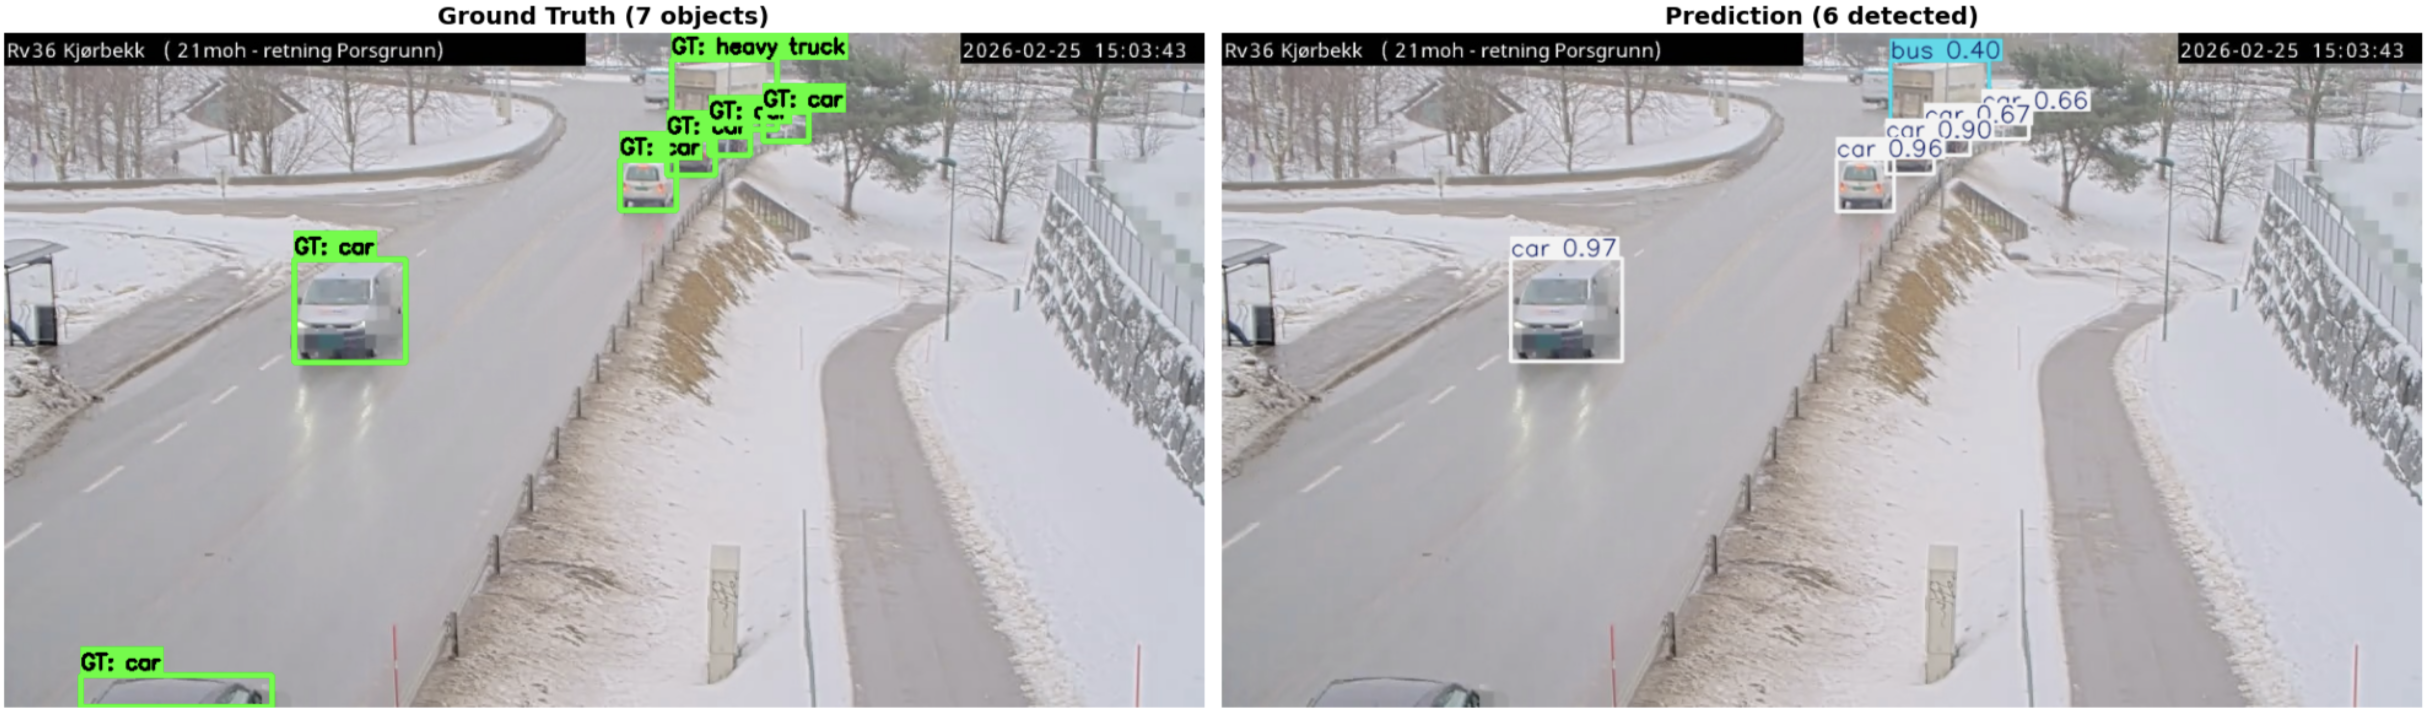
\includegraphics[width=1\linewidth]{project//images/FN_crop.png}
    \caption{\textbf{False Negative:} A car entering the frame from the bottom is annotated, but not predicted.}
    \label{fig:FN_crop}
\end{figure}


\begin{figure}[H]
    \centering
    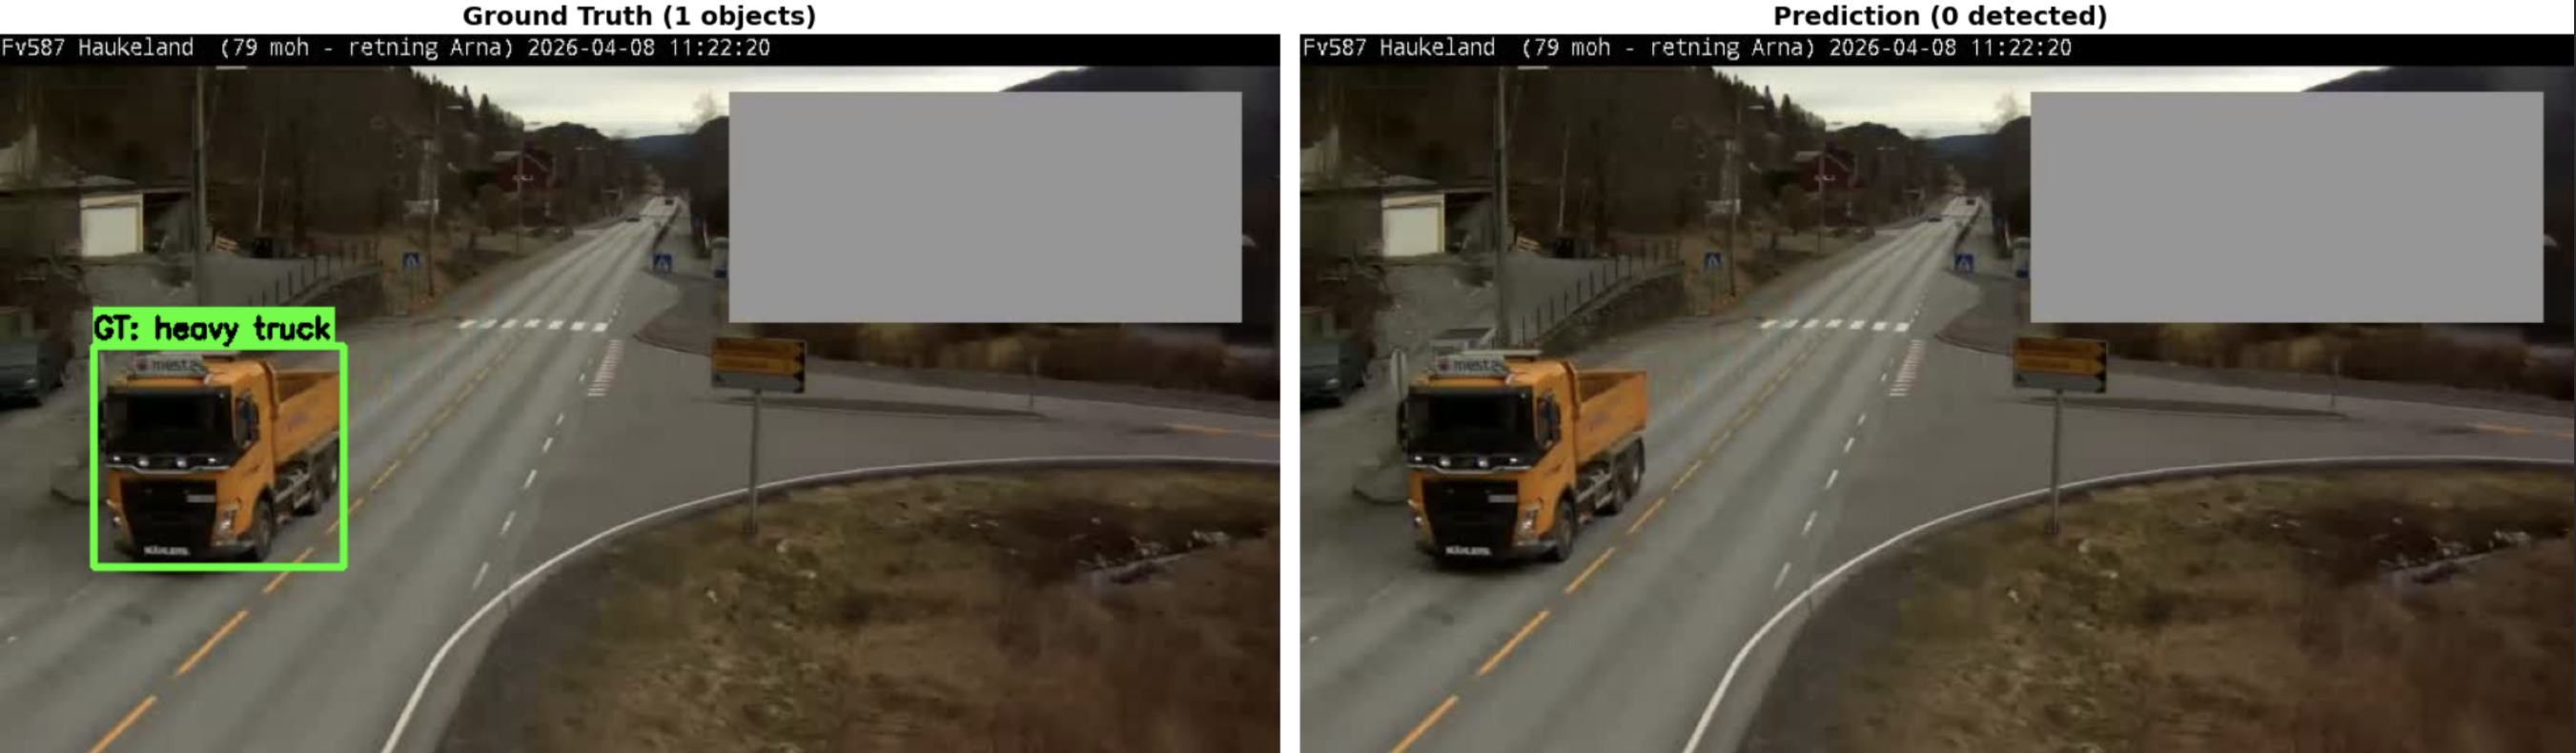
\includegraphics[width=1\linewidth]{project//images/FN_why.png}
    \caption[\textbf{False Negative:} A heavy truck is clearly present, but the model misses it.]{\textbf{False Negative:} A heavy truck is clearly present, but the model misses it. Further investigation reveals that the model actually predicted light truck, but with under 5\% confidence, way below the threshold of 25\%.}
    \label{fig:FN_why}
\end{figure}

\begin{figure}[H]
    \centering
    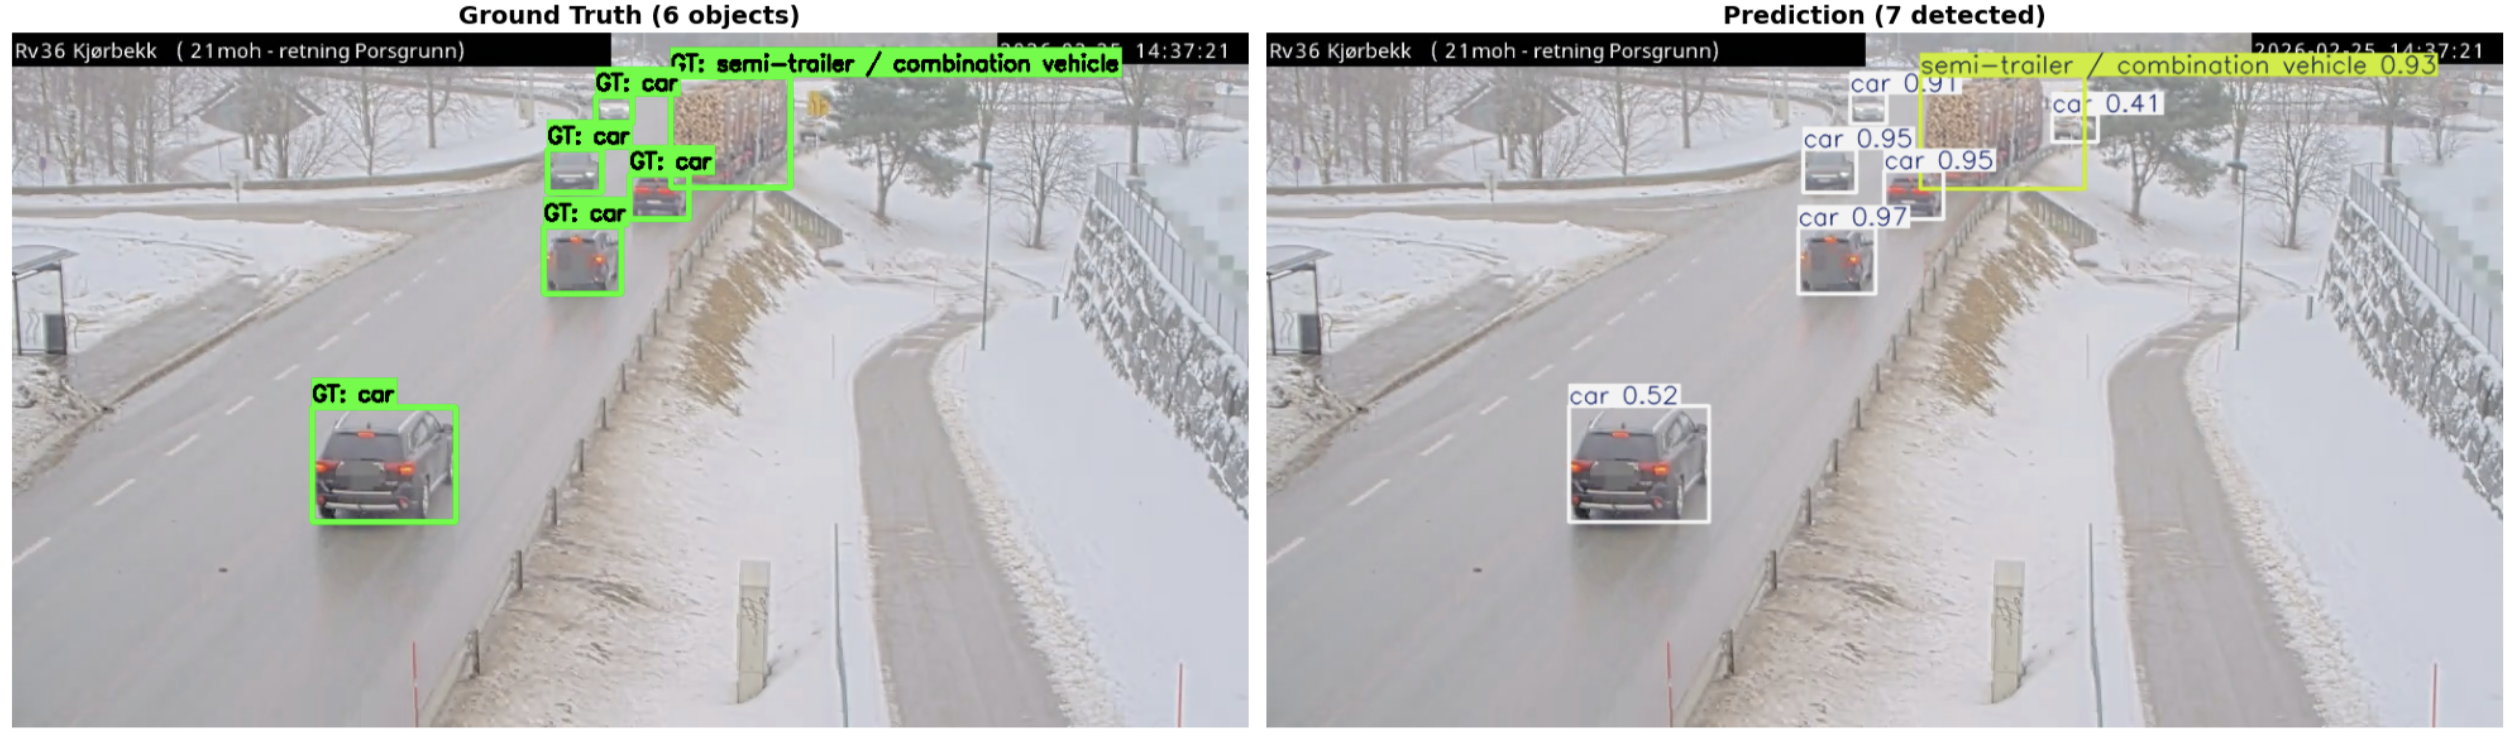
\includegraphics[width=1\linewidth]{project//images/FP_occlusion.png}
    \caption{\textbf{False Positive:} The car on the top right was too far away from the region of interest, so it was not annotated. The model predicts it regardless, even though it is far away and partially occluded.}
    \label{fig:FP_occlusion}
\end{figure}


\begin{figure}[H]
    \centering
    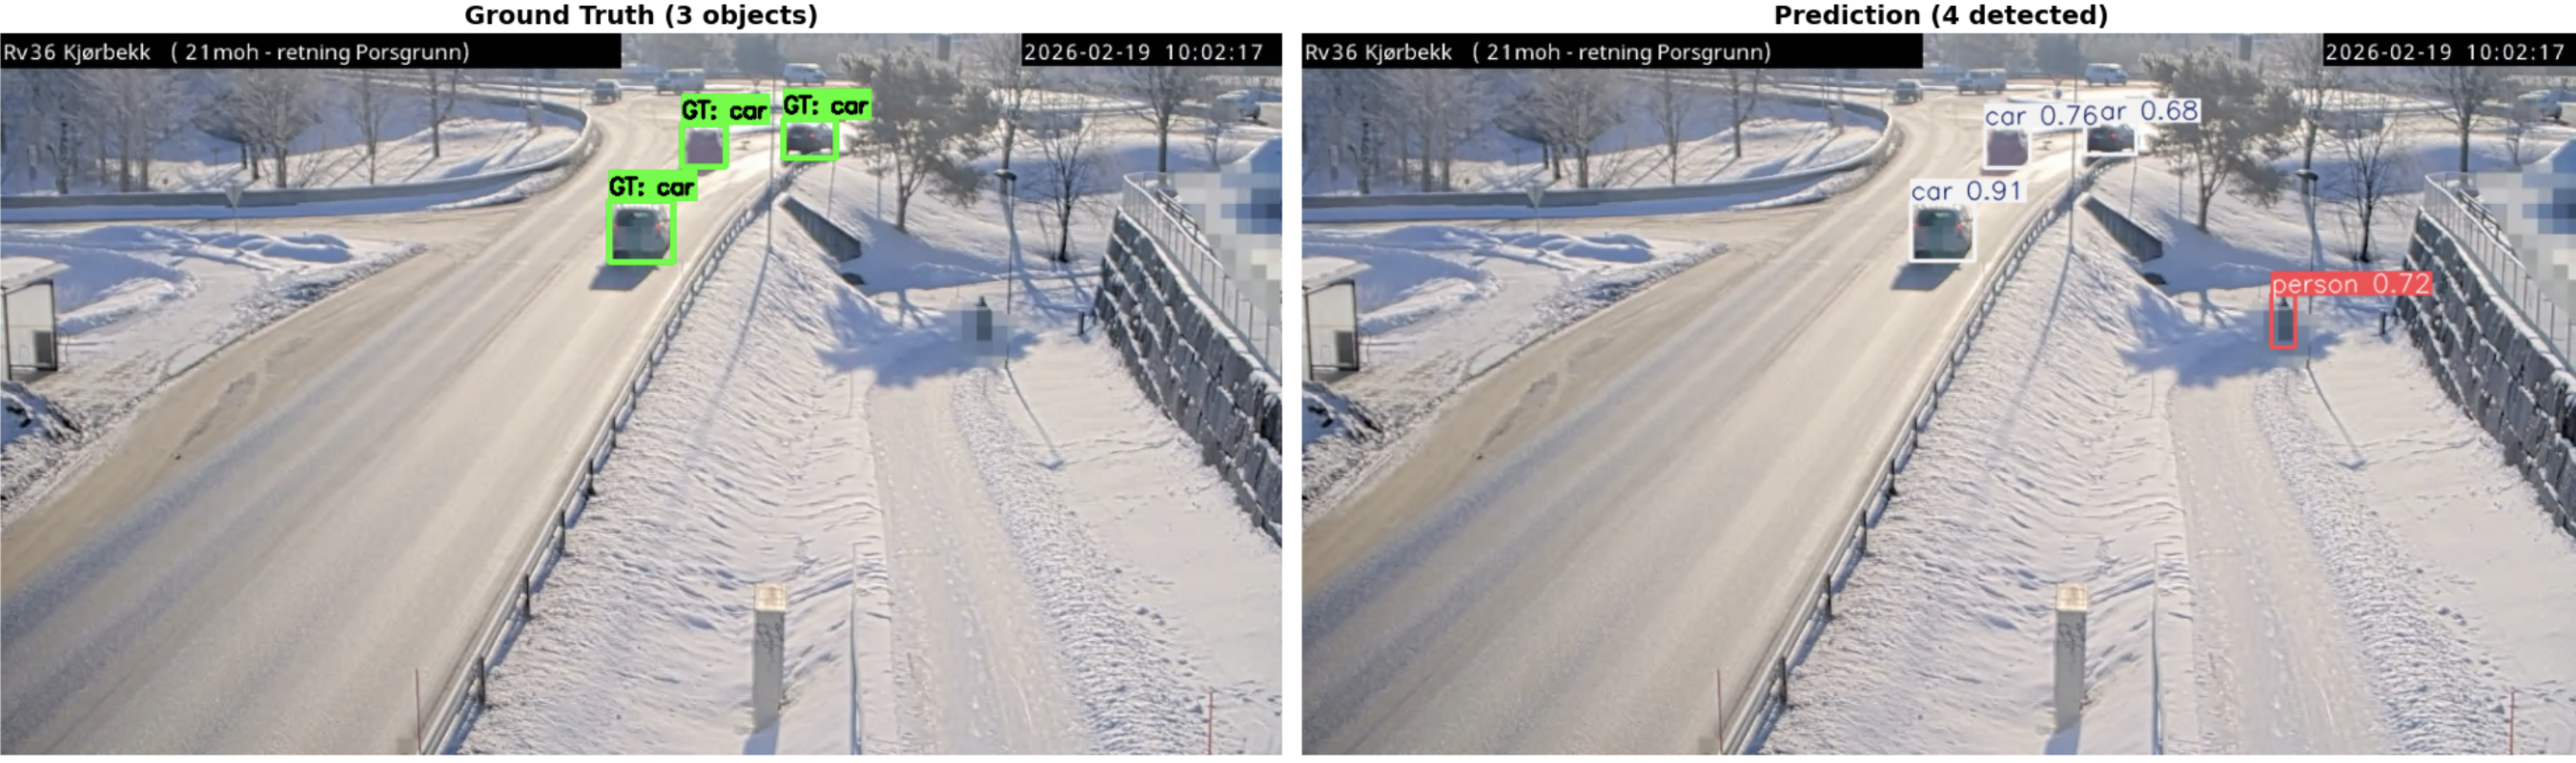
\includegraphics[width=1\linewidth]{project//images/FP_blurry.png}
    \caption{\textbf{False Positive:} A person has gone unnoticed during the annotation, but the model still predicts it.}
    \label{fig:FP_blurry}
\end{figure}

\begin{figure}[H]
    \centering
    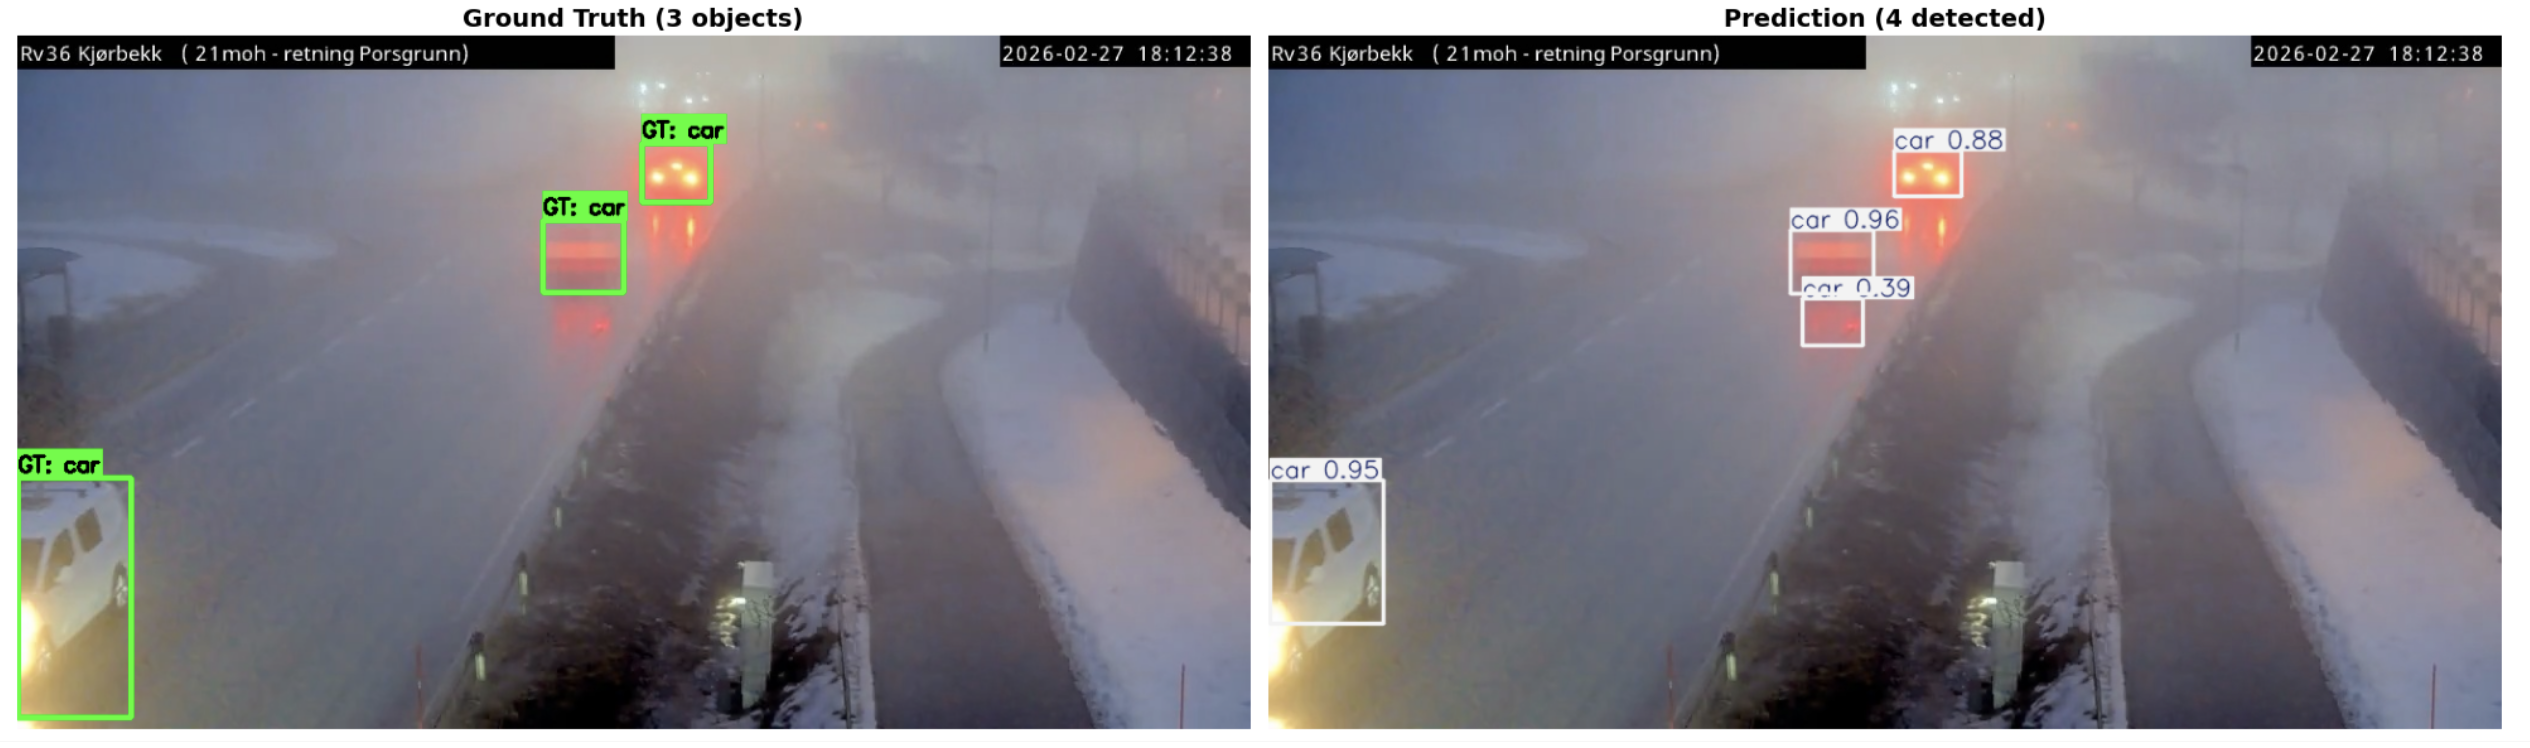
\includegraphics[width=1\linewidth]{project//images/FP_light.png}
    \caption{\textbf{False Positive:} Due to challenging lightning, the model predicts the reflection of a car as an object.}
    \label{fig:FP_light}
\end{figure}

\begin{figure}[H]
    \centering
    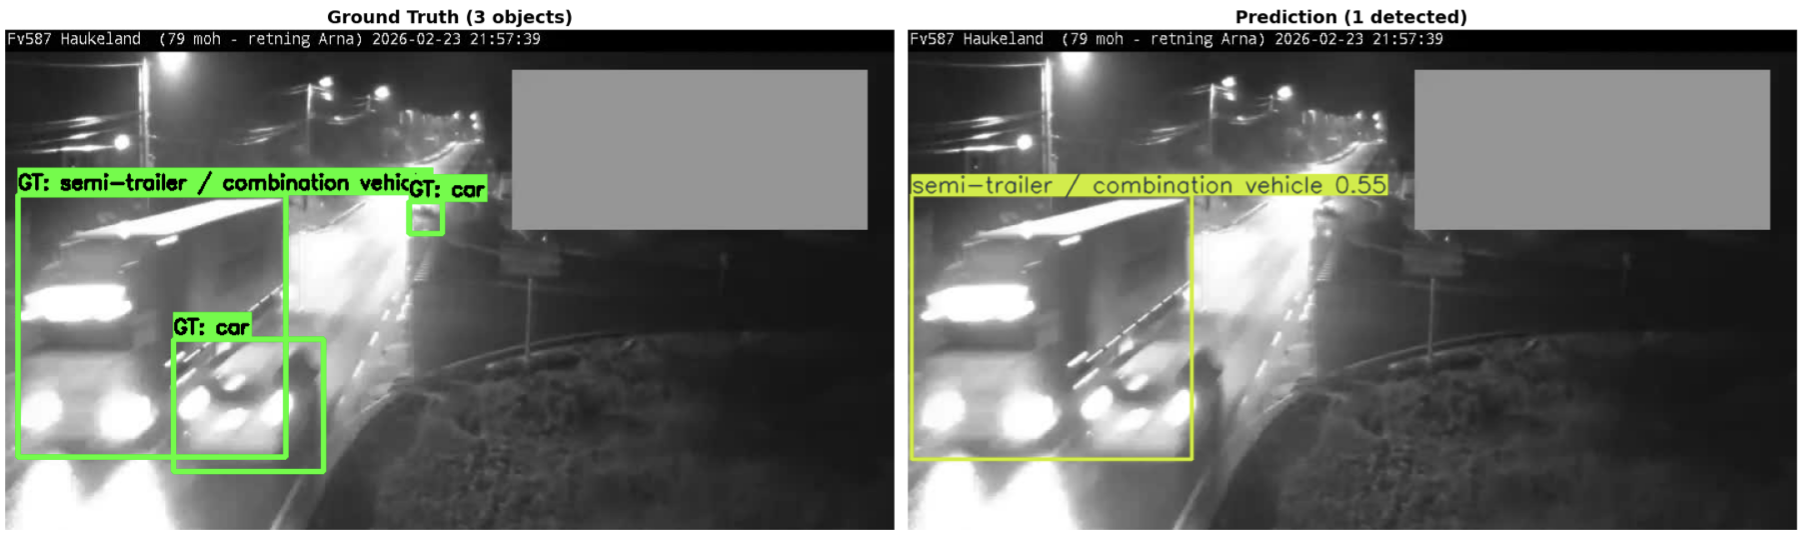
\includegraphics[width=1\linewidth]{project//images/night_pred.png}
    \caption{\textbf{False Negative:} Missed detection at nighttime.}
    \label{fig:FN_night}
\end{figure}


